\newpage
\section{Verifizierung und Ergebnisse}
\subsection{Planung}
Zur Verifizierung der in C++ implementierten Verzerrung wurde ein Auswertungsskript in MATLAB erstellt. Die Grundidee der Verifizierung ist, dass für einfache Szenen die Verzerrung des Bildes durch Änderung des verfolgten Lichtstrahls ungefähr äquivalent mit der Interpolation eines unverzerrten Bildes, gerendert durch die \texttt{PerspectiveCamera} des pbrt, sein sollte.
Dies wird auf zwei Arten überprüft:
\begin{enumerate}
	\item Das durch \texttt{DistortionCamera} gerenderte Bild, wird mit dem gegebenen Polynom \textbf{entzerrt} und mit dem von \texttt{PerspectiveCamera} gerenderten Bild verglichen.
	\item Das durch \texttt{PerspectiveCamera} gerenderte Bild wird mit dem gegebenen Polynom \textbf{verzerrt} und mit dem von \texttt{DistortionCamera} gerenderten Bild verglichen.
\end{enumerate}

Als Grundlage des Tests wird das in Abbildung \ref{fig:test_img} dargestellte Punkteraster angenommen. 

\begin{figure}[h]
	\centering
	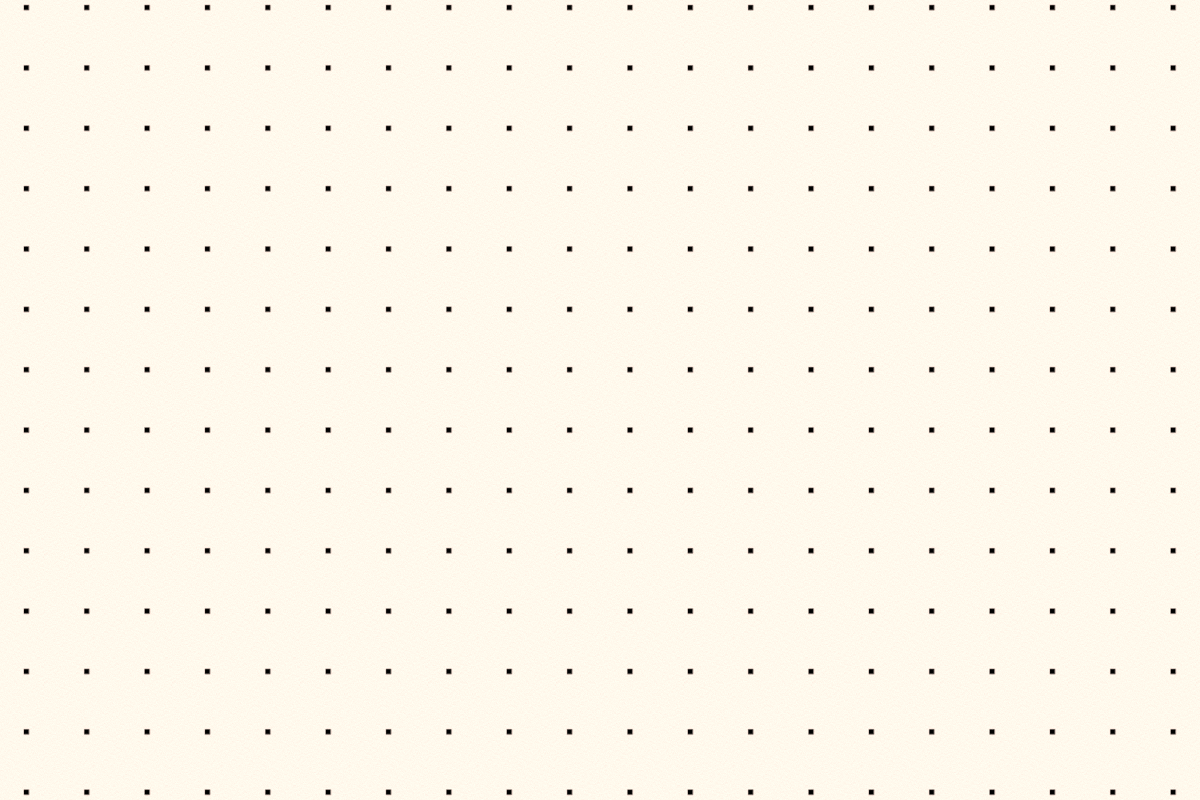
\includegraphics[width=0.5\textwidth]{img/dot_perspective.png}
	\caption{Testbild: Punkteraster, gerendert mit pbrt \texttt{PerspectiveCamera}}
	\label{fig:test_img}
\end{figure}

Es wird zum einen die Differenz zwischen den Ergebnissen von pbrt und Matlab optisch auf systematische Fehler überprüft, zum anderen wird die Peak-Signal-to-Noise-Ratio (kurz \textbf{PSNR}) als quantitative Fehlermetrik genutzt.
Diese ergibt sich aus der maximalen Intensität des Bildes $I_\text{max}$ und dem Mean-Square-Error $\text{MSE}$:
\begin{equation}
	PSNR = 10\cdot \log_{10} (I_\text{max}^2/\text{MSE})
\end{equation}
Es sei hier erwähnt, dass die PSNR keine Metrik für Bildqualität ist, sondern für die Fehlerabschätzung beliebiger Signale genutzt wird \cite{Akramullah2014}.

Da die Verzerrung und Entzerrung keine chromatischen Aberrationen mit einbezieht, wird jeder Farbkanal mit der gleichen Verzerrung berechnet. Aus diesem Grund werden zum Vergleich der Bilddaten lediglich Grauwerte gezeigt.

\subsection{Implementierung in Matlab}
Die Ver- und Entzerrung in Matlab erfolgt durch eine Funktion namens \texttt{distortImage}. Diese nimmt als Eingangswerte ein Eingangsbild und ein Array von Polynomkoeffizienten sowie mehrere optionale Parameter entgegen. Die optionalen Übergabeparameter erlauben ein Verschieben des Bildmittelpunktes und die Auswahl zwischen Ver- und Entzerrung des Bildes mit den gegebenen Koeffizienten. 
Als erster Schritt werden jedem Bildpunkt die normierten X und Y Koordinaten zugewiesen und in ein Format gebracht, welches der Interpolant entgegen nimmt:
\begin{lstlisting}[style=Matlab-editor,basicstyle=\mlttfamily]
%% Bestimmung der normierten X und Y-Koordinaten mit Center-Offset
xRange = scale*((-(Lx-1)/2:(Lx-1)/2)-cx);
yRange = scale*((-(Ly-1)/2:(Ly-1)/2)-cy);
[X,Y] = meshgrid(yRange,xRange);
\end{lstlisting}
Anschließend werden für jeden Bildpunkt neue Koordinaten nach Verzerrung durch das gegebene Polynom bestimmt:
\begin{lstlisting}[style=Matlab-editor,basicstyle=\mlttfamily]
%% Berechne das Verzerrungspolynom und verzerrte XY Coordinaten
function [distortedX,distortedY] = distortXY(X,Y,polyCoefficients)
  R = sqrt(X.^2+Y.^2);
  R_factor = zeros(size(R));
  for index = 1:numel(polyCoefficients)
    exponent = index-1;
    R_factor = R_factor+polyCoefficients(index)*R.^(exponent);
  end
  distortedX = X.*R_factor;
  distortedY = Y.*R_factor;
end
\end{lstlisting}
Je nach Ver- oder Entzerrung wird von den normierten in die verzerrten Koordinaten interpoliert oder umgekehrt.
\begin{lstlisting}[style=Matlab-editor,basicstyle=\mlttfamily]
%% Berechnung der X,Y Position nach Ver/Entzerrung
if strcmp(mode,'distort')
	img_vector = reshape(img,pixelCount,1);
	P = cat(3,distortedX,distortedY);
	%%
	P = reshape(P,pixelCount,2);
	interpolant = scatteredInterpolant(P,img_vector,'linear','none');
	imgOut = interpolant(X,Y);
elseif strcmp(mode,'undistort')
	imgOut = interpn(X,Y,img,distortedX,distortedY,'linear',NaN);
end
\end{lstlisting}


\subsection{Region-Of-Interest}
\label{sec:roi}
Die Interpolatoren sind so konfiguriert, dass die Bildbereiche außerhalb des gültigen Wertebereiches einen NaN Wert erhalten. Alle Werte, die erfolgreich interpoliert werden, bilden die Region-Of-Interest (kurz \textbf{ROI}) für einen Vergleich der Bilder.
\begin{lstlisting}[style=Matlab-editor,basicstyle=\mlttfamily]
%% Bestimmung der Region of Interest für Entzerrung
roi = ~isnan(imgOut);
\end{lstlisting}
Der für die Verzerrung eingesetzte \texttt{ScatteredInterpolant} interpoliert zwischen gegebenen Bildpunkten auf Basis einer Triangulation der Punkte. Die gesamte Basis interpolierbarer Punkte ist dabei die konvexe Hülle der Gesamtpunkte (vgl. Abbildung~\ref{fig:convex_hull}). Einige dieser Punkte lägen bei einer unverzerrten Kamera außerhalb des Bildes, daher kann die Interpolation in diesem Bereich keine sinnvollen Werte liefern. Im Folgenden wird der fehlerhafte Bereich dennoch als Teil der ROI beachtet, da die Bestimmung einer passenden konkaven Hülle den Umfang dieser Arbeit überschreiten würde.
\begin{figure}[h]
	\begin{minipage}{.3\textwidth}
		\centering
		
\includegraphics[width=\textwidth]{img/pc.png}
		\caption{Punktwolke von Bildpunkten}
		\label{fig:pointcloud}
	\end{minipage}
	\begin{minipage}{.3\textwidth}
	\centering
	
\includegraphics[width=\textwidth]{img/distortedpc.png}
	\caption{Punktwolke verzerrter Bildpunkte}
	\label{fig:distorted_pointcloud}
	\end{minipage}
	\begin{minipage}{.3\textwidth}
		\centering
		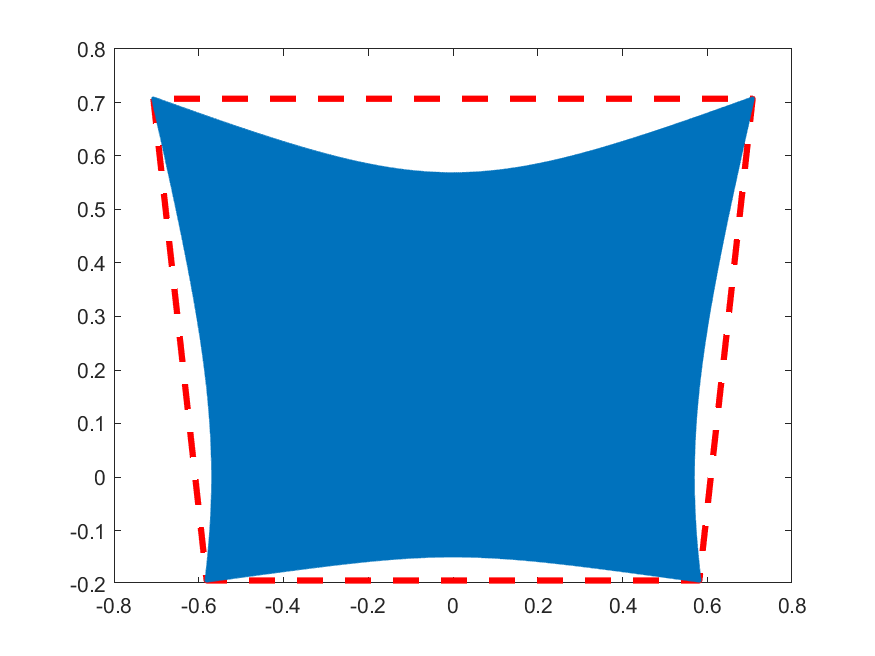
\includegraphics[width=\textwidth]{img/convexpc.png}
		\caption{Konvexe Hülle der verzerrten Bildpunkte}
		\label{fig:convex_hull}
	\end{minipage}
\end{figure}

\subsection{Vergleich}
Die Basis des folgenden Vergleiches bildet eine Reihe von gerenderten Verzerrungen:
\begin{description}
	\item[Verzerrungsmodell] Poly3-Modell
	\item[Bildmittelpunkt-Offset] $X$: $0$, $Y$: $0.5$
	\item[Koeffizient $k_1$] Von $k_1 = 0.0125$ wiederholt verdoppelt bis $k_1 = 0.4$.
\end{description}
Sowohl das Testbild aus Abbildung~\ref{fig:test_img}, die gerenderten Testbilder und die daraus in Matlab entstandenen Bilder sind im dieser Arbeit zugehörigen Git-Repository \cite{git-Distortion_Camera} zu finden. Beispiele sind in Abbildung~\ref{fig:rendered_examples} zu sehen.
\begin{figure}[h]
	\centering
	\begin{minipage}{.3\textwidth}
		\centering
		\includegraphics[width=\textwidth]{img/pbrtDistorted/{dots_poly3_0.0125_cxy_0_0.5}.png}
		\caption*{$0.0125$}
		\label{fig:render_0_0125}
	\end{minipage}
	\begin{minipage}{.3\textwidth}
		\centering
		\includegraphics[width=\textwidth]{img/pbrtDistorted/{dots_poly3_0.1_cxy_0_0.5}.png}
		\caption*{$0.1$}
		\label{fig:render_0_1}
	\end{minipage}
	\begin{minipage}{.3\textwidth}
		\centering
		\includegraphics[width=\textwidth]{img/pbrtDistorted/{dots_poly3_0.4_cxy_0_0.5}.png}
		\caption*{$0.4$}
		\label{fig:render_0_4}
	\end{minipage}
	\caption{Gerendertes Testmuster mit verschiedenen Werten für $k_1$}
	\label{fig:rendered_examples}
\end{figure}
Abbildung~\ref{fig:difference_example} zeigt die Wertedifferenz des perspektivisch gerenderten Bildes und der Entzerrung. Auf diesem Bild, wie auch den restlichen Testbildern ist kein systematischer Unterschied bei der Positionierung der Punkte zu erkennen. 
Es lässt sich vermuten, dass die Fehler an den Kanten lediglich durch die Interpolation entstehen. 
In Abbildung~\ref{fig:difference_dist_0_4} ist im oberen Bildrand zu erkennen, wie Punkte welche durch den pbrt abgebildet werden, durch Matlab nicht korrekt interpoliert werden können. Hier trifft die in Abschnitt~\ref{sec:roi}  beschriebene fehlerhafte Interpolation innerhalb der konvexen Hülle ein. 
\begin{figure}[h]
		\centering
		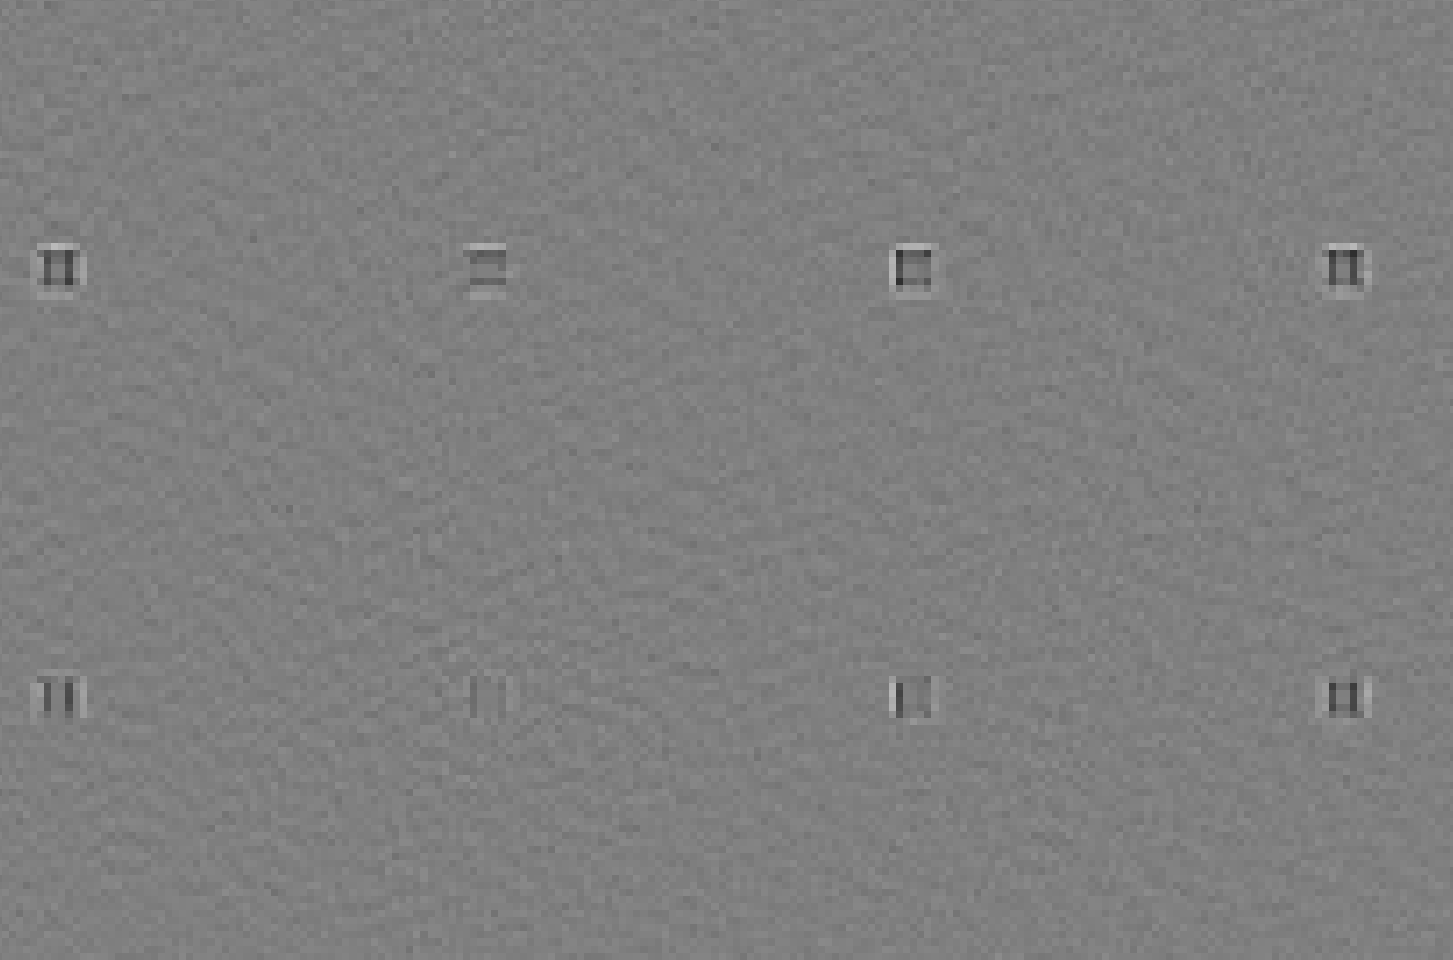
\includegraphics[width=.5\textwidth]{img/error_shape.png}
		\caption{Wertedifferenz zwischen perspektivischem Render und Entzerrung (vergrößert)}
		\label{fig:difference_example}
\end{figure}

\begin{figure}[h]
		\centering
		\begin{minipage}{.49\textwidth}
			\centering
			\includegraphics[width=\textwidth]{img/differenceDistorted/{dots_poly3_0.4_cxy_0_0.5}.png}
			\subcaption{Differenz Matlab- und pbrt-Verzerrung}
			\label{fig:difference_dist_0_4}
		\end{minipage}
		\begin{minipage}{.49\textwidth}
			\centering
			\includegraphics[width=\textwidth]{img/differenceUndistorted/{dots_poly3_0.4_cxy_0_0.5}.png}
			\subcaption{Differenz Matlab-Entzerrung und Test-Bild}
		\end{minipage}
	\caption{Wertedifferenzen von Ent-/Verzerrung mit $k_1 = 0.4$ Mittleres Grau = Kein Fehler, Schwarz/Weiß: Vorzeichenbehafteter Fehler}
	\label{fig:difference_0_4}
\end{figure}

Tabelle~\ref{tbl:comparison} zeigt den Einfluss der Stärke der Verzerrung auf die Ähnlichkeit der Ergebnisse von Matlab und pbrt. Grundsätzlich ergibt sich aus einer stärkeren Verzerrung ein größerer Interpolationsfehler. 
Die PSNR-Werte bei Tests mit anderen Verzerrungsmodellen liegen im gleichen Wertebereich (ca. $37-40\text{ dB}$ bei geringer Verzerrung). Bei der Verschiebung des perspektivischen Bildes um einen halben Pixel ergibt sich beim Vergleich mit der unverschobenen Version eine PSNR von $32.22 \text{ dB}$.
Insgesamt kann daher davon ausgegangen werden, dass das entwickelte pbrt Modell die Verzerrung korrekt berechnet.

\begin{table}
	\centering
\begin{tabular}{|c|c|c|c|c|}
	\hline 
	\rule[-1ex]{0pt}{2.5ex}  & \multicolumn{2}{c|}{Entzerrung} & \multicolumn{2}{c|}{Verzerrung}  \\ 
	\hline 
	\rule[-1ex]{0pt}{2.5ex} $k_1$ & $\text{PSNR}/\text{dB}$ & $|e_\text{MAX}|$ & $\text{PSNR}/\text{dB}$ & $|e_\text{MAX}|$ \\ 
	\hline 
	\rule[-1ex]{0pt}{2.5ex} 0.0125 & 40.02 & 0.2366 & 39.90 & 0.2701 \\ 
	\hline 
	\rule[-1ex]{0pt}{2.5ex} 0.025 & 40.00 & 0.2488 & 39.93 & 0.2588 \\ 
	\hline 
	\rule[-1ex]{0pt}{2.5ex} 0.05 & 39.72 & 0.2675 & 39.88 & 0.2918 \\ 
	\hline 
	\rule[-1ex]{0pt}{2.5ex} 0.1 & 39.59 & 0.2667 & 40.08 & 0.2907 \\ 
	\hline 
	\rule[-1ex]{0pt}{2.5ex} 0.2 & 38.86 & 0.3357 & 38.87 & 0.9769 * \\ 
	\hline 
	\rule[-1ex]{0pt}{2.5ex} 0.4 & 35.42 & 0.5514 & 33.16 & 0.9865 * \\ 
	\hline 
\end{tabular} 

\caption{Auswertung der Reihe von Bildern mit PSNR und maximalem Absolutfehler (höchster Bildwert ist 1). Mit * markierte Werte stammen von der ungenauen ROI (Abschnitt~\ref{sec:roi})}
\label{tbl:comparison}
\end{table}
